\chapter{Technologiewahl}
Im Kapitel der Technologiewahl werden einige aktuell erhältliche Smartwatch Modelle mit den theoretischen Daten verglichen, allegemeine Eigenschaften aufgeführt und die Entwicklerfreundlichkeit bewertet. Aufgrund der Bewertung von aufgestellten Kriterien werden ein bis zwei Uhren ausgewählt für die Arbeit.

\section{Allgemeine Eigenschaften}
Heute (Januar 2016) sind weitgehends alle erhältlichen tragbaren Computer am Handgelenk vom Smartphone abhängig, deshalb bieten sie nur einen kleinen Mehrwert. Sie können zwar viel mehr als nur die Zeit anzeigen, jedoch sehr beschränkt und zum grössten Teil wird das Mobiltelefon benötigt. Nachrichten, Termine und einkommende Telefonate anzeigen, aber ein Gespräch kann nur mit den wenigsten Geräten geführt werden, wie z.B. der Apple Watch. Mit den meisten Smartwatches können Nachrichten gelesen, jedoch nicht beantwortet werden, da diese über keine virtuelle Tastatur verfügen. Falls doch geschieht dies hauptsächlich über die Spracheingabe. Mit dem integrierten Touchscreenkeyboard, stellt die Samsung Gear S dar die einzige Ausnahme dar.

Smartwatches wollen die Gesundheit fördern, etliche davon messen den Puls, zählen die Schritte und erfassen zurückgelegte Wegstrecke. Weitere Apps erlauben den Schlaf zu überwachen, zur Bewegung aufzufordern bei langer inaktivität und den Kalorienbedarf und Verbrauch berechnen. Durch die genauen Daten haben Amateursportler eine praktische Hilfe am Handgelenk, um ihren Körper fit zu halten. Für ambitionierte Sportler ist der Funktionsumfang no zu gering.

Manche Uhren der Hersteller Apple, LG, Samsung und Alcatel messen den Puls fast Elektrokardiogramm-genau. Apple arbeitet bereits an einem Elektrokardiogramm (EKG) Armband, welches Daten per Ultraschall übermitteln soll. Das Band ermittelt die Herzströme über zwei angebrachte Elektroden. Dies ermöglicht der Apple Smartwatch als mobiles EKG bereitzustehen\footnote{vgl. \url{http://www.smartwatch.de/news/neues-apple-watch-armband-mit-ultraschall-ekg-geplant}, 20.11.2015}.

Ein grosse, fast alle betreffende, Schwachstelle von Smartwatches sind ihre leistungsschwachen Akkumulatoren. Durchschnittlich erreichen die Uhren eine Laufzeit von knapp 24 Stunden bei geringer Nutzung.

Applikationen welche einen grossen Mehrwert bringe gibt es no zu wenige. Zum heutigen Zeitpunkt stellt sich heraus, dass die Minicomputeruhren überwiegend als Erweiterungsbildschrim des Smartphones dient. Wenige Geräte werkeln autonom, wie zum Beispiel die Samsung, jedoch bleiben die meisten ein verlängerter Arm des dazugehörigen Mobiltelefons. Dies liegt daran, weil die smarten Uhren noch Heute in den Kinderschuhen stecken.

\section{Kandidaten}
\begin{table}[H]
\begin{minipage}{\textwidth}
\centering
\begin{tabular}{|>{\columncolor[gray]{0.8}}p{4cm}|p{4cm}|p{4cm}|p{4cm}|}
\hline

  & 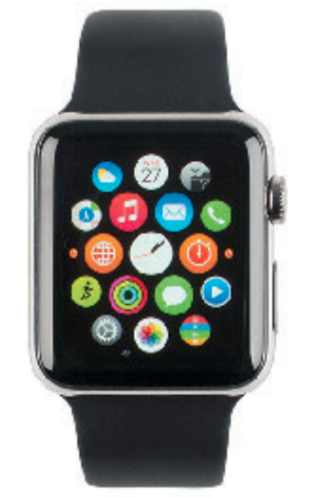
\includegraphics[width=2.5cm]{98_Bilder/06_Smartwatch_Produkte/AppleWatch}
  & 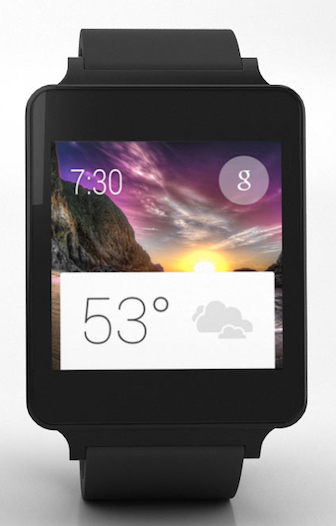
\includegraphics[width=2.5cm]{98_Bilder/06_Smartwatch_Produkte/LGGWatch}
  & 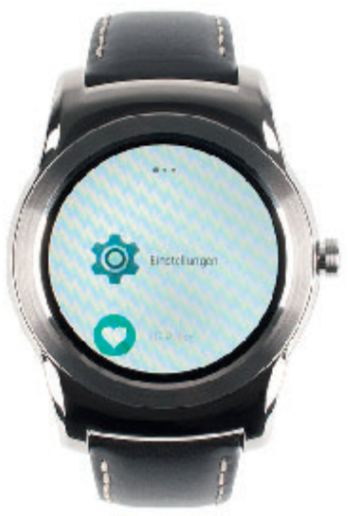
\includegraphics[width=2.5cm]{98_Bilder/06_Smartwatch_Produkte/LGWatchUrbane} \\ \hline
\textbf{Smartwatch}
  & Apple Watch\footnote{vgl. Stiftung Warentest Magazin, Ausgabe: 10/2015}
  & LG G Watch\footnote{vgl. Modul BTI7302 Evaluation Wearables, 27.06.2015}
  & LG Watch Urbane\footnote{vgl. Stiftung Warentest Magazin, Ausgabe: 10/2015} \\ \hline
\textbf{Betriebsystem}
  & WatchOS
  & Android Wear
  & Android Wear \\ \hline
\textbf{Funktionen}
  & gut
  & befriedigend
  & befriedigend \\ \hline
Nachrichten
  & empfangen möglich, \newline senden per Sprachnachricht, \newline Emojis senden
  & empfangen möglich, \newline senden per Sprachnachricht
  & empfangen möglich, \newline senden per Sprachnachricht \\ \hline
Telefonieren
  & führen von Gespräche
  & nur Notifikation
  & nur Notifikation \\ \hline
Display
  & 42mm 312x390px \newline 38mm 272x340px
  & 1.65 Zoll 280x280px
  & 1.3 Zoll 320x320px \\ \hline
\textbf{$\varnothing$ Akkulaufzeit}
  & 19h
  & 30h
  & 20h \\ \hline
\textbf{Datensendungsverhalten}
  & verschlüsselt
  & verschlüsselt
  & verschlüsselt \\ \hline
\textbf{Smartphone-Betriebssystem}
  & ab iOS 8.2
  & ab Android 4.3 \newline ab iOS 8.2
  & ab Android 4.3 \newline ab iOS 8.2 \\ \hline
\textbf{Pulsmesser}
  & optischer Pulsmesser
  & kein Pulsmesser
  & optischer Pulsmesser \\ \hline
\textbf{Gesamteindruck}
& bestes Display \newline viele Funktionen \newline \textbf{befriedigend - gut}
& Always-On Display \newline befriedigender Akku \newline \textbf{befriedigend}
& rundes Display \newline edle Verarbeitung \newline \textbf{befriedigend} \\ \hline
\end{tabular}
\caption{Technische Daten von Smartwatches - Teil 1}
\end{minipage}
\end{table}

\begin{table}[H]
\begin{minipage}{\textwidth}
\centering
\begin{tabular}{|>{\columncolor[gray]{0.8}}p{4cm}|p{4cm}|p{4cm}|p{4cm}|}
\hline

  & 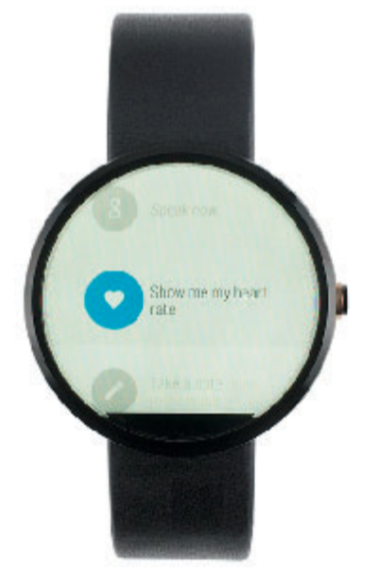
\includegraphics[width=2.5cm]{98_Bilder/06_Smartwatch_Produkte/MotorolaMoto360}
  & 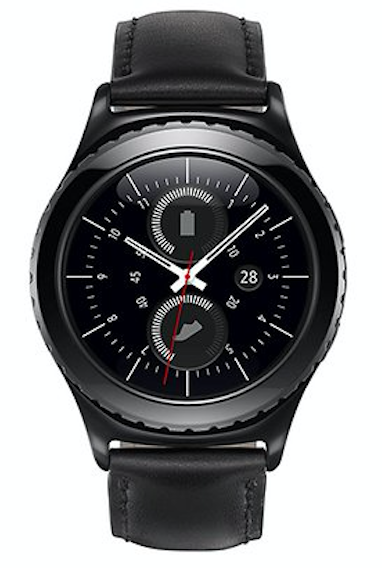
\includegraphics[width=2.5cm]{98_Bilder/06_Smartwatch_Produkte/SamsungGearS2}
  & 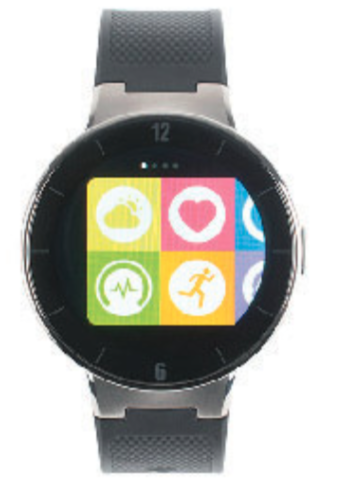
\includegraphics[width=2.5cm]{98_Bilder/06_Smartwatch_Produkte/AlcatelOnetouchWatch} \\ \hline
\textbf{Smartwatch}
  & Motorola Moto 360\footnote{Referenz: Modul BTI7302 Evaluation Wearables, Michael Fankhauser und Sathesh Paramasamy, Ausgabe: 27.06.2015}
  & Samsung Gear S2\footnote{Referenz: \url{https://www.androidpit.de/samsung-gear-s2-test}, Stand: 27.12.2015}
  & Alcatel Onetouch Watch\footnote{Referenz: Stiftung Warentest Magazin, Ausgabe: 10/2015} \\ \hline
\textbf{Betriebsystem}
  & Android Wear
  & Tizen
  & proprietäres Alcatel OS \\ \hline
\textbf{Funktionen}
  & befriedigend
  & gut
  & befriedigend \\ \hline
Nachrichten
  & empfangen möglich, \newline senden per Sprachnachricht
  & empfangen möglich, \newline senden möglich
  & empfängt nur Kurznachrichten \\ \hline
Telefonieren
  & nur Notifikation
  & nur Notifikation \newline bei eSIM Variante möglich
  & nur Notifikation \\ \hline
Display
  & 1.57 Zoll 360x290px
  & 1.2 Zoll 360x360px
  & 1.3 Zoll 320x320px \\ \hline
\textbf{$\varnothing$ Akkulaufzeit}
  & 10h
  & 38h
  & 20h \\ \hline
\textbf{Datensendungsverhalten}
  & verschlüsselt
  & verschlüsselt
  & unverschlüsselt \\ \hline
\textbf{Smartphone-Betriebssystem}
  & ab iOS 8.2
  & ab Android 4.4
  & ab Android 4.3 \newline ab iOS 7 \\ \hline
\textbf{Pulsmesser}
  & optischer Pulsmesser
  & optischer Pulsmesser
  & optischer Pulsmesser \\ \hline
\textbf{Gesamteindruck}
& bestes Display \newline meiste Funktionen \newline \textbf{befriedigend}
& Intuitive Lünette \newline gute Akkuleistung \newline \textbf{befriedigend - gut}
& schwaches Display \newline mangelhafte Datenübertragung \newline \textbf{mangelhaft} \\ \hline
\end{tabular}
\caption{Technische Daten von Smartwatches - Teil 2}
\end{minipage}
\end{table}

\section{Entscheid Smartwatch}
Wenn der Funktionsumfang betrachtet wird, wäre eine Apple Watch oder die Samsung Gear S2 die bevorzugte Wahl gewesen. Die Samsung ist erst seit Oktober 2015 erhältlich, folglich fiel diese Aufgrund des späten Erscheinungsdatum und dessen Samsung proprietären Betriebssystem Tizen aus dem Katalog. Die Apple Watch wurde nicht gewählt, weil die Entwicklung sich auf die Apple spezifische Programmiersprache Swing beschränkt. Ein weitere Entscheidungspunkt ist, dass der Markt aus einem Produkt besteht, wenn man die Modelle Watch und Watch Sport und die Grössen, 38mm und 42mm, nicht unterscheidet, da diese sich nur optisch voneinander unterscheiden.
Ausgewählt wurden zwei Produkte, welche nicht sehr aufgefallen sind: Die \textbf{LG G Watch} und die \textbf{Motorola Moto 360}. Als erste auf dem Markt erhältliche Android Wear Smartwatch, wurde die LG G Watch ausgewählt. Der eingebaute Snapdragon 400 Prozessor rechnet mit 1,2 GHz, hat 512MB RAM und hat ein rechteckigen Bildschrim, welcher die Funktion biete immer eingeschaltet zu sein. Wichtiger Pluspunkt ist, die LG Datenuhr kann über USB gedebugged werden. Dies erleichtert die Entwicklung von Applikation. Um ein Android Wear Vergleichsobjekt zu erhalten, kam die neuere Motorola Moto 360 zusätzlich in die Entscheidung. Diese arbeitet mit einem Texas Instrument OMAP 3 Prozessor mit 1 GHz, hat ebenfalls 512MB RAM und hat einen runden Touchscreen. Mehrwert der Moto 360 zur G Watch sind, ein eingebautes WLAN Modul, Lichtsensor, Pulssensor und eine physische Taste. Bedauerlicherweise kann sie nur über Bluetooth gedebbugt werden, was viel Zeit beansprucht um entwicklte Apps zu übertragen. Durch die Entscheidung für Android Wear liegt der Schwerpunkt auf der Entwicklungsprache JAVA.
